\chapter{UML diagramy a obrázky}
\section{Use cases}
\label{use_cases}

\begin{figure}[H]
\begin{center}
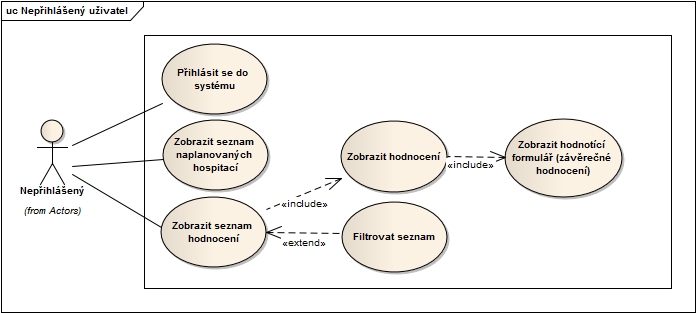
\includegraphics[width=12cm]{figures/actor_base}
\caption{Use case - nepřihlášený uživatel}
\label{fig:actor_base}
\end{center}
\end{figure}

\begin{figure}[H]
\begin{center}
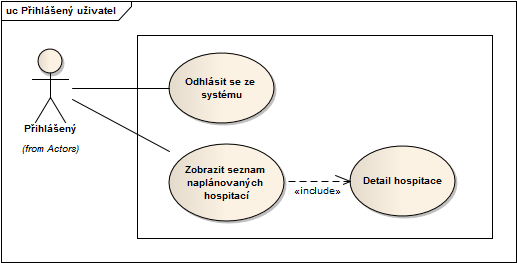
\includegraphics[width=12cm]{figures/actor_logged}
\caption{Use case - přihlášený uživatel}
\label{fig:actor_logged}
\end{center}
\end{figure}

\begin{figure}[H]
\begin{center}
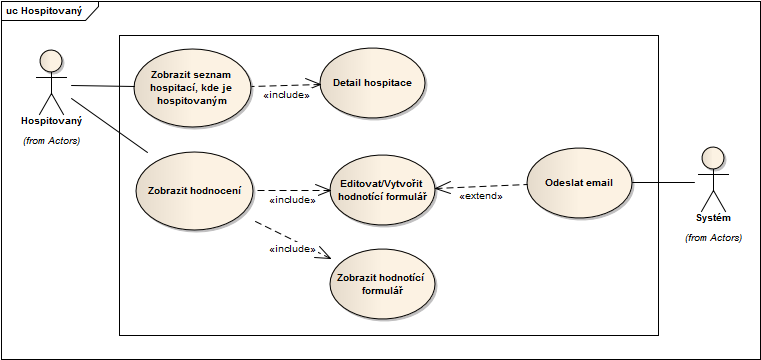
\includegraphics[width=12cm]{figures/actor_observed}
\caption{Use case - hospitovaný}
\label{fig:actor_observed}
\end{center}
\end{figure}

\begin{figure}[H]
\begin{center}
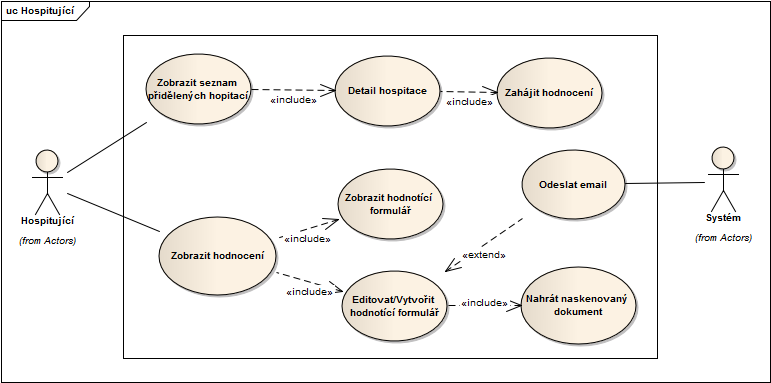
\includegraphics[width=12cm]{figures/actor_observer}
\caption{Use case - hospitující}
\label{fig:actor_observer}
\end{center}
\end{figure}

\begin{figure}[H]
\begin{center}
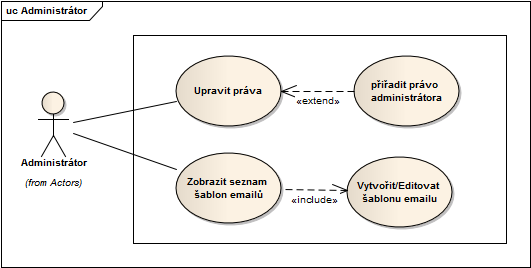
\includegraphics[width=12cm]{figures/actor_root}
\caption{Use case - administrátor}
\label{fig:actor_root}
\end{center}
\end{figure}

\begin{figure}[H]
\begin{center}
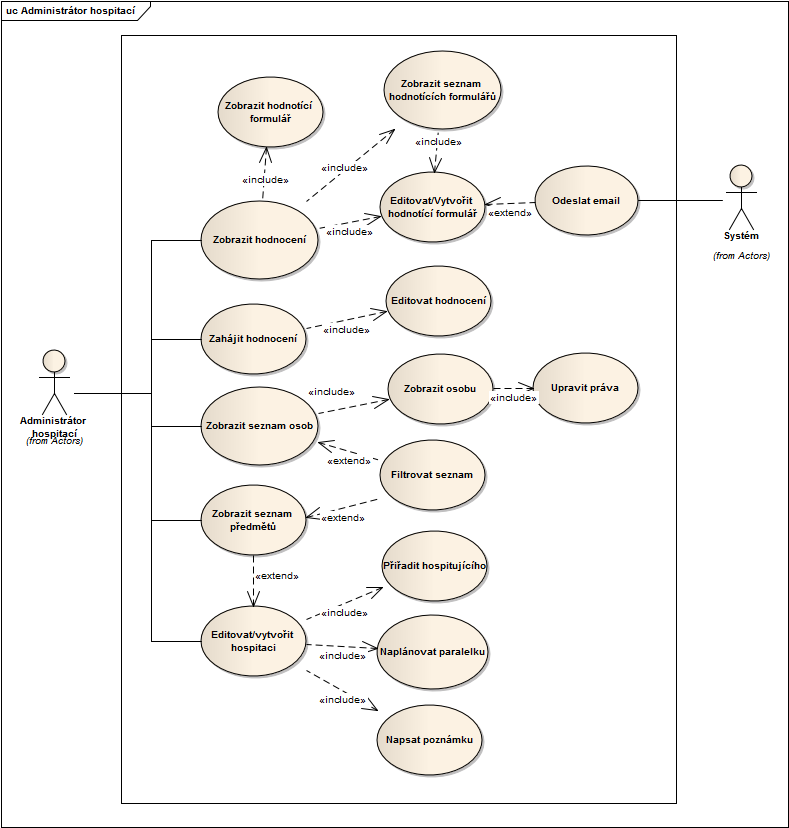
\includegraphics[width=14cm]{figures/actor_admin}
\caption{Use case - administrátor hospitací}
\label{fig:actor_admin}
\end{center}
\end{figure}


\chapter{Dynamické formuláře}
\begin{table}[h]
\begin{center}
\begin{tabular}{|l|c|l|}

\hline
\textbf{Typ} & \textbf{Návratová hodnota} & \textbf{Popis} \\ \hline
label &  & textový popisek \\\hline
integer & číslo & vstupní element pro čísla \\ \hline
text & text & formulář pro psaní textů \\\hline
text/file & text & formulář pro psaní textů s možností \\ & &  nahrání souboru s naskenovaným formulářem \\\hline
ranking\_table &  & tabulka pro hodnocení, může obsahovat několik \\ & & elementů typu \textit{ranking} \\\hline
column\_table & & tabulka do které se vkládají jiné elementy \\ & &  po sloupcích \\\hline
ranking & [A,B,C,D,E,F] & vstupní element pro zadávaní známkování  \\ & &   od A do F \\\hline
ranking\_scale & & tabulka s hodnotící stupnicí \\\hline
note & text & vstupní element pro napsání textové poznámky \\\hline

\end{tabular}
\caption{Seznam podporovaných typů elementů}
\label{tab:elements}
\end{center}
\end{table}

\begin{figure}[H]
\begin{center}
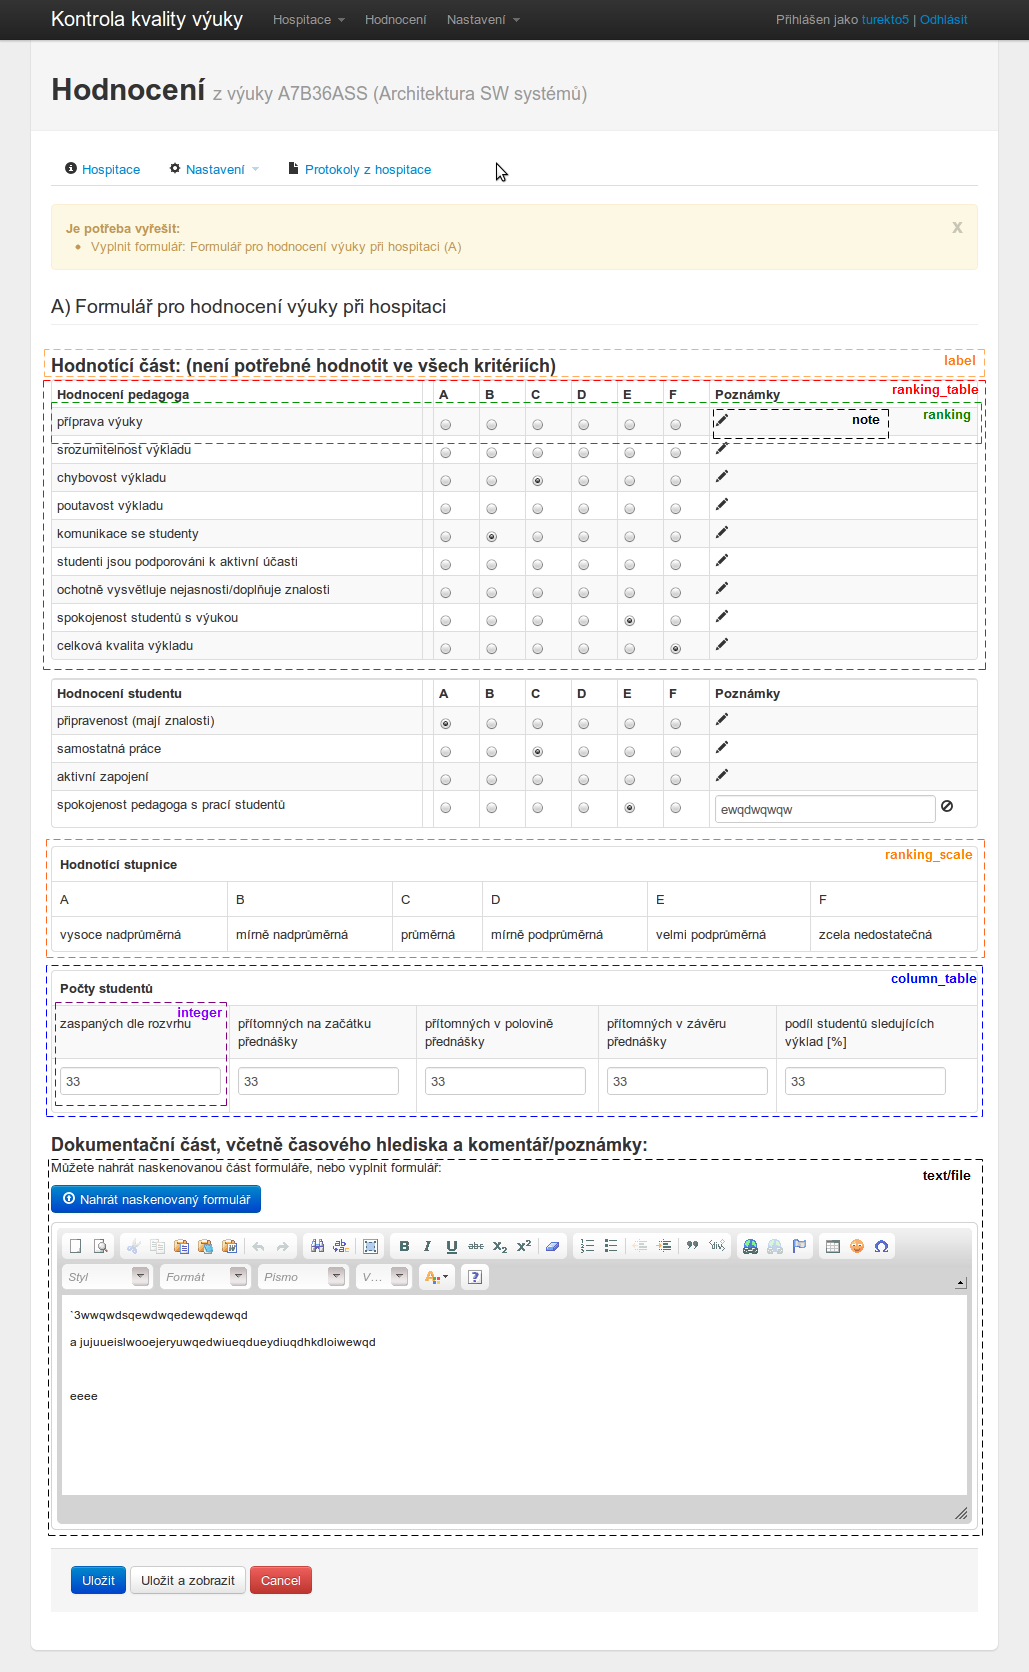
\includegraphics[width=14cm]{figures/form_A}
\caption{Hodnotící formulář A}
\label{fig:actor_admin}
\end{center}
\end{figure}

%*****************************************************************************
\chapter{Instalační příručka}
\textbf{\large Tato příloha velmi žádoucí zejména u softwarových implementačních prací.}

%*****************************************************************************
\chapter{Obsah přiloženého CD}
\begin{figure}[h]
	\dirtree{%
		.1 /.
		.2 readme.txt\DTcomment{stručný popis obsahu CD}.
		.2 src/\DTcomment{zdrojové kódy aplikace}.
		.2 prototyp/\DTcomment{prototyp aplikace}.
		.3 src/\DTcomment{zdrojové kódy prototypu}.
		.3 BP.pdf\DTcomment{text prototypu ve formátu PDF}.
		.2 thesis/\DTcomment{zdrojová forma práce ve formátu
\LaTeX{}}.
 		.3 figures/\DTcomment{obrázky pro text práce}.
		.2 text/\DTcomment{zdrojová forma práce ve formátu}.
		.3 thesis.pdf\DTcomment{text práce ve formátu PDF}.
	}
	\caption{Obsah CD}
\label{tree:obsah_cd}
\end{figure}
%$ tree . >tree.txt
